\chapter{Implementierung}
Wie eben bereits erwähnt, wird in dieser Arbeit die Crate \texttt{gdbstub} verwendet. Sie implementiert das GDB RSP, sodass nicht jedes Detail der Paketverarbeitung manuell umgesetzt werden muss. Stattdessen bietet die Crate Schnitstellen, über die das Zielsystem sein spezifisches Verhalten bereitstellt. Eine minimale Integration erfordert lediglich, dass man die Traits Connection und Target, sowie eine Form des Event Loops implementiert. In Connection wird die Kommunikationsart, hier der serielle Port, definiert. Der Target Trait dient als primäre Brücke zwischen dem RSP und dem Systemspezifischen Code. Hier wird definiert, wie das System während der Debugging Session kontrolliert und modifiziert werden kann. Der Event Loop verarbeitet die eingehenden Pakete und leitet sie an die entsprechenden Schnittstellen weiter, schickt aber auch Pakete an das RSP zurück bei Events, die durch zum Beispiel Systemstopp ausgelöst werden \cite{gdbstub}.

\section{Connection}
Der Connection Trait ist die Schnittstelle zur Kommunikation. Da D3OS eine No-Std Umgebung ist, muss Connection manuell implementiert werden. Dazu müssen die Methoden \texttt{write()} und \texttt{flush()} mit dem Verhalten unserer Kommunikationsart befüllt werden \cite{gdbstub}. Es wurde sich hier für einen polling-basierten seriellen Port entschieden, da D3OS schon die Schnittstelle für den seriellen Port bereitstellt und die Rechner der Abteilung Betriebssysteme über einen solchen Port verfügen. Da es sich bei polling-baseriten Verfahren um blockierende I/O handelt, muss hier zusätzlich der Trait ConnectionExt implementiert werden, der neben den eben genannten Methoden weiterhin \texttt{read} und \texttt{peek} benötigt \cite{gdbstub}.

\section{BlockingEventLoop}
Der Event Loop ist einerseits dafür verantwortlich, eingehende Pakete auszuwerten und die richtigen Funktionen aufzurufen, andererseits aber auch dafür den Systemzustand an GDB zu übermitteln, wenn bestimmte Ereignisse passieren. Die Crate bietet dafür zwei Möglichkeiten an. Mit der \texttt{GdbStubStateMachine} hat man selbst die volle Kontrolle über den Event Loop. Für Implementierungen, die keinen extra Thread aufwenden wollen beziehungsweise können oder Interrupt getriebene I/O verwenden, ist das die bevorzugte Variante \cite{gdbstub}.\\ 
Da hier aber schon blockierende I/O verwendet wird und beim debuggen auch nicht die maximale Effizienz des Systems benötigt wird, wird hier der \texttt{BlockingEventLoop} verwendet. Wie der Name schon sagt blockiert der Event Loop so lange, bis entweder neue Daten anliegen oder der Stub ein Event and GDB melden muss. Dazu muss die Methode \texttt{wait\_for\_stop\_reason} implementiert werden. Außerdem erwartet der BlockingEventLoop Trait auch, dass die Methode \texttt{on\_interrupt} implementiert wird \cite{gdbstub}.

\subsection{wait\_for\_stop\_reason}
Diese Methode wird aufgerufen nachdem die \texttt{resume} Methode des Zielsystems aufgerufen wurde. Sie soll blockieren bis entweder neue Daten über \texttt{Connection} gesendet wurden oder das System gestoppt ist \cite{gdbstub}. Dazu läuft eine Endlosschleife, in der zuerst mit \texttt{peek} überprüft wird, ob neue Daten anliegen und falls ja werden diese gelesen und über \texttt{Event::IncomingData(byte)} an die entsprechenden Methoden weitergeleitet. Danach wird überprüft, ob der \texttt{DebugState} ein \texttt{DebugEvent} gespeichert hat. Falls ja wird basierend auf dem \texttt{DebugEvent} entschieden, welche \texttt{StopReason} an GDB übermittelt wird.

\subsection{on\_interrupt()}
Diese Funktion verarbeitet den \texttt{CtrlC} Befehl von GDB. Dieser Befehl soll den Programmfluss anhalten und GDB die Kontrolle geben \cite{gdb}. Dazu werden die Interrupts ausgeschaltet und alle Threads außer dem Stub-Thread angehalten. Außerdem wird ein \texttt{DebugEvent::CtrlC} gesetzt. Danach wird zum Stub-Thread gewechselt und es können neue Befehle eingegeben werden. Das Programm wird hier aber nicht durch eine Exception unterbrochen. Der \texttt{CtrlC} Befehl wird erst verarbeitet, wenn der Scheduler zum Stub-Thread wechselt. Dieser hält das Programm dann an und wartet auf neue Befehle. Da erst zum Stub-Thread gewechselt werden muss, befindet sich der angehaltene Thread immer im Kontext der \texttt{thread\_switch} Funktion. 

\section{DebugState} 
Für die Kommunikation zwischen den verschiedenen Komponenten und dem Stub wird ein globaler Zustand verwendet. Dieser ist notwendig, da Exceptions im Kontext des ausgeführten Threads auftreten und behandelt werden, die Kommunikation mit GDB jedoch durch den Stub-Thread erfolgt. Der globale Zustand speichert das zuletzt aufgetretene \texttt{DebugEvent}, damit es vom Event Loop verarbeitet werden kann, aber auch Listen der gesetzten Breakpoints. Da auf den Zustand aus verschiedenen Threads zugegriffen wird, werden die einzelnen Felder über Mutexe synchronisiert. 

\section{Target}
Der Target Trait ist eine zentrale Schnittstelle der Crate. Dazu stellt \texttt{gdbstub} verschiedene Handler-Methoden bereit, die vom Zielsystem implementiert werden müssen. Hier wird unterschieden zwischen Single-Thread- und Multi-Thread-Systemen. Da D3OS mehrere Threads unterstützt, werden in dieser Arbeit die Schnittstellen für Multi-Thread-Zielsysteme implementiert. Eine minimale Implementierung erfordert hier die Methoden \texttt{read\_registers}, \texttt{write\_registers}, \texttt{read\_addrs}, \texttt{write\_addrs} und \texttt{list\_active\_threads}. Das ist aber um diverse weitere Funktionen erweiterbar.\\
Außerdem müssen hier auch architekturspezifische Informationen wie Pointergröße und Registerlayout angegeben werden \cite{gdbstub}. Für viele der gängigen Architekturen, unter anderem auch das von D3OS verwendete x86\_64, gibt es aber eine zusätzliche Crate \texttt{gdbstub\_arch}, in welcher die erforderlichen Informationen bereits implementiert sind \cite{gdbstub-arch}.

\subsection{Inlineable Dyn Extension Traits}
Das GDB RSP ist sehr umfangreich und bietet viele verschiedene optionale Funktionen an. Damit nicht jeder Entwickler jedes optionale Feature implementieren muss, verwendet \texttt{gdbstub} optionale Trait Erweiterungen. Da die klassischen Ansätze optionale Methoden zu implementieren Nachteile hinsichtlich der Performance oder Ergonomie mit sich bringen, verwendet \texttt{gdbstub} eine Technik die der Autor \textit{Inlineable Dyn Extension Traits} (IDETs) nennt. Dadurch lassen sich die Traits problemlos erweitern und der Compiler erkennt Dinge wie gegenseitig abhängige Methoden bereits zur Compilezeit, ohne dass Unmengen von Cargo Features benutzt werden müssen. Die genaue Funktionsweise der IDETs kann in der Dokumentation der Crate nachgelesen werden \cite{gdbstub}.

\subsection{read\_registers}
Die Methode \texttt{read\_registers} bekommt als Parameter eine Thread-ID und eine Struct, deren Felder mit dem Registerzustand des Threads befüllt werden müssen, übergeben \cite{gdbstub}. Dazu werden zuerst die Threadinformationen durch den Scheduler abgerufen. Über die Thread Struct von D3OS kann der zuvor gespeicherte Stack Pointer \texttt{old\_rsp0} des Threads abgefragt werden. Da beim Verarbeiten von GDB Anfragen der Thread mit dem Stub aktiv ist, liegt der gesamte Threadkontext wie in Grafik \ref{grafik_1} auf dem Stack. Dabei zeigt \texttt{old\_rsp0} auf den gespeicherten Wert von \texttt{GSBASE}, also genau den Anfang des Bereichs, in dem der Registerzustand gespeichert ist. Die Registerwerte liegen als 64 Bit Integer auf dem Stack. Daher kann \texttt{old\_rsp0} als Pointer auf ein Array interpretiert werden. Im Falle von \texttt{read\_registers} wird von diesem Array eine Kopie erstellt, da hier nur gelesen werden muss. Außerdem erwartet GDB noch den Stack Pointer, der nach Wiederherstellung des Threadzustands gültig ist. Dieser kann berechnet werden, indem \texttt{old\_rsp0} um die Größe eines 64 Bit Integers, multipliziert mit der Anzahl der auf dem Stack liegenden Werte, erhöht wird. Mit dem Array und dem berechneten Stack Pointer Wert kann anschließend die übergebene Struct befüllt werden, über die der Registerzustand an GDB gemeldet werden kann.

\begin{figure}[h]
\centering
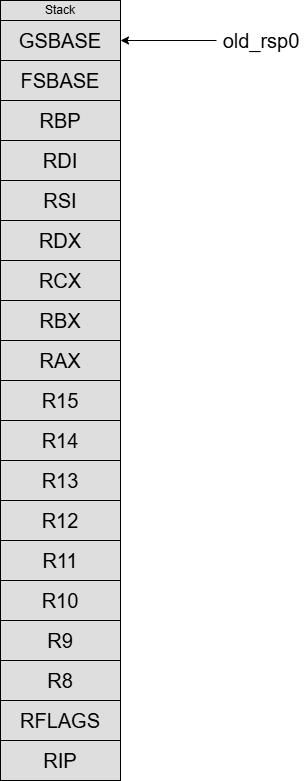
\includegraphics[width=0.6\linewidth,height=0.5\textheight,keepaspectratio]{img/stackframe.drawio}
\caption{Registerwerte auf dem Stack}
\label{grafik_1}
\end{figure}

\begin{codeblock}{gdbtarget.rs}{Rust}
\begin{rustcode}
pub fn thread_context_from_rsp(rsp: VirtAddr) -> Option<ThreadContext> {
	if rsp.is_null() {
		return None;
	}
	let raw_rsp0 = rsp.as_u64();
	let registers = unsafe { 
		(raw_rsp0 as *const [u64; THREAD_REG_COUNT]).read() 
	};
	let restored_rsp = raw_rsp0 + (THREAD_REG_COUNT * size_of<u64>()) as u64;
	Some(ThreadContext {
		registers,
		rsp: restored_rsp,
	})
}
\end{rustcode}
\end{codeblock}

\subsection{write\_registers}
Die Methode \texttt{write\_registers} ist ähnlich zu \texttt{read\_registers} aufgebaut. GDB übergibt hier wieder eine Thread-ID und eine Struct mit Registerwerten. Im Gegensatz zu \texttt{read\_registers} muss jedoch der Threadzustand mit den Werten aus der Struct überschrieben werden \cite{gdbstub}. Dazu werden wieder die Threadinformationen durch den Scheduler abgerufen und über \texttt{old\_rsp0} der Speicherbereich auf dem Stack als Array interpretiert. Für \texttt{write\_registers} wird aber keine Kopie erstellt, sondern eine mutable Referenz auf den Speicherbereich. Dadurch können die Werte auf dem Stack direkt verändert werden. Diese Werte werden beim nächsten Kontextwechsel in die Register geladen.

\begin{codeblock}{gdbtarget.rs}{Rust}
\begin{rustcode}
pub fn mut_thread_context_from_rsp(rsp: VirtAddr) -> Option<ThreadContextMut> {
	// Das meiste ist gleich wie bei der Read-Only Version,
	// der Hauptunterschied ist in folgender Zeile
	let registers = unsafe { 
		&mut *(raw_rsp0 as *mut [u64; THREAD_REG_COUNT])
	};
}
\end{rustcode}
\end{codeblock}

\subsection{read\_addrs}
GDB übergibt hier eine virtuelle Adresse, eine Thread-ID und ein Array \texttt{data}, das mit den Daten an der jeweiligen Adresse befüllt werden muss \cite{gdbstub}. Da der Stub vorerst nur im Kernel arbeitet, muss hier kein neuer Adressraum geladen werden. Man kann also direkt über die Bytes, die an der virtuellen Adresse stehen, iterieren und die Daten in das Array schreiben. Die Funktion meldet bei erfolgreicher Ausführung \texttt{data.len()} and GDB.

\subsection{write\_addrs}
Die Methode \texttt{write\_addrs} funktioniert ähnlich zu \texttt{read\_addrs}, das \texttt{data} Array hält hier aber die Daten, die an die Adresse geschrieben werden sollen \cite{gdbstub}. Die Daten an der Adresse werden also beim iterieren überschrieben statt gelesen.

\subsection{list\_active\_threads}
GDB übergibt hier eine Callback Funktion, an die die IDs aller aktiven Threads übergeben werden müssen \cite{gdbstub}. Der Scheduler verwaltet die aktiven Threads in Listen, die nach Zustand sortiert sind. Durch diese Listen kann iteriert werden, um die IDs der Threads, die nicht im Zustand \texttt{Exited} sind, abzurufen. Die IDs werden an die Callback Funktion übergeben und dadurch an GDB weitergeleitet.

\section{Software Breakpoints}
Breakpoints sind eine zentrale Funktion eines Debuggers um Programme richtig untersuchen zu können. Software Breakpoints können durch Einsetzen einer Architekturspezifischen Instruktion verwendet werden und lösen eine Exception aus, wenn diese Instruktion ausgeführt wird \cite{intel-sdm}. \texttt{gdbstub} bietet jeweils eine Funktion zum setzen und entfernen von Software Breakpoints. Das genaue Verhalten des Systems, nachdem ein Breakpoint getroffen wurde, muss jedoch von einer extra Handler Funktion implementiert werden.

\subsection{add\_sw\_breakpoint}
Der Stub bekommt hier von GDB eine virtuelle Adresse und ein \texttt{BreakpointKind} übergeben \cite{gdbstub}. \texttt{BreakpointKind} wird normalerweise benutzt, um auf bestimmten Architekturen zu entscheiden, welche Art Breakpoint eingesetzt werden soll  \cite{gdb}. Bei \texttt{x86\_64} gibt es aber nur eine Software Breakpoint Instruktion, also ist dieser Parameter hier egal \cite{intel-sdm}. Um Software Breakpoints zu verwalten, wird eine Liste im \texttt{DebugState} gespeichert, die die Adressen und Originalbytes für die Breakpoints sichert. Da es kein Limit für gleichzeitig aktive Software Breakpoints gibt, wird als Liste hier ein Vector verwendet, damit sie dynamisch wachsen kann. Zuerst wird überprüft, ob in der Liste von Breakpoints bereits ein Breakpoint an der übergebenen Adresse steht. Falls ja, wird GDB direkt informiert, dass dort ein Breakpoint steht. Das ist die gleiche Antwort, die auch beim erfolgreichen Einsetzen eines neuen Breakpoints geschickt wird. Wenn die Adresse noch nicht in der Liste ist, wird erst das erste Byte der Originalinstruktion an der Stelle ausgelesen. Danach wird an diese Stelle die Breakpointinstruktion \texttt{0xCC} geschrieben \cite{intel-sdm}. Dann muss das Byte der Originalinstruktion mit der Adresse zusammen in die Liste mit Breakpoints geschrieben werden, damit später die richtige Instruktion wieder an die Adresse geschrieben werden kann.

\subsection{remove\_sw\_breakpoint}
Die Methode bekommt die gleichen Parameter wie \texttt{add\_sw\_breakpoint} \cite{gdbstub}. Hier wird in der Liste nach dem Eintrag mit der richtigen Adresse gesucht. Der Eintrag wird gelöscht und die Originalinstruktion wieder an die Adresse geschrieben.

\subsection{Breakpoint Handler}
Wenn eine Breakpoint Instruktion ausgeführt wird, löst das System einen INT3 Interrupt, beziehungsweise eine Breakpoint Exception, aus \cite{intel-sdm}. D3OS verwendet zum behandeln von Exceptions den IDT (Interrupt Descriptor Table) aus der \texttt{x86\_64} Crate \cite{x86-64}. Dadurch können über ein Makro sehr einfach Handler-Funktionen für bestimmte Exceptions registriert werden. Das Makro bekommt die IDT Instanz, die Handler-Funktion und den Index des Interrupts, der behandelt werden soll, übergeben. Der Index ist hier drei. Die Handler-Funktion bekommt dann ein \texttt{InterruptStackFrame} übergeben, welches die folgende Werte enthält \cite{x86-64}:

\begin{itemize}
\item Instruction Pointer
\item Code Segment
\item RFlags
\item Stack Pointer
\item Stack Segment
\end{itemize}

Damit die Threads nicht weiterlaufen, müssen beim Betreten des Breakpoint-Handlers Interrupts ausgeschaltet werden. Das reicht aber nicht, da die Threads nach Verlassen des Handlers trotzdem weiter laufen. Sie werden aber nicht mehr richtig durch den Scheduler verwaltet, was dazu führt, dass die Threads fälschlicherweise terminieren. Um das zu vermeiden wird hier ein neuer Thread Zustand \texttt{DebugStopped} hinzugefügt. Im Breakpoint-Handler werden alle Threads, die als Zustand \texttt{Ready} haben, zu \texttt{DebugStopped} geändert und der \texttt{blocked\_list} hinzugefügt, damit sie nicht vom Scheduler ausgewählt werden können sobald der Handler verlassen wird. Der Thread, in dem der Stub läuft, darf aber nicht gestoppt werden. Außerdem muss der Stub an GDB melden, dass ein Breakpoint getroffen wurde. Dazu wird ein \texttt{DebugEvent::SwBreakpoint} in den \texttt{DebugState} geschrieben. Da der Breakpoint-Handler durch den Thread, der die Exception ausgelöst hat, aufgerufen wird, muss zum Schluss noch zum Stub-Thread gewechselt werden. Er ist der einzige Thread mit Zustand \texttt{Ready}, weshalb hier einfach \texttt{switch\_thread\_from\_interrupt()} aufgerufen werden kann, weil es nur einen Thread gibt, in den der Scheduler wechseln kann. Der Thread mit dem Stub läuft dann in einem  Busy Loop im Exceptionkontext, bis neue Befehle von GDB ankommen. Außerdem muss der Handler den Instruction Pointer noch reduzieren.

Der \texttt{InterruptStackFrame}, den der Handler übergeben bekommt, ist nur ein Wrapper für die Werte, damit nicht versehentlich etwas geändert wird. Er kann jedoch in ein \texttt{InterruptStackFrameValue} konvertiert werden, in dem sich die Werte dann ändern lassen. Beim Testen hat sich jedoch rausgestellt, dass das nur Kopien der Werte sind und Änderungen nur die Instanz betreffen. Deswegen werden Änderungen von Flags oder dem Instruction Pointer nicht übernommen.

Weil beim Interrupt andere Werte gepusht werden, als bei einem Thread Switch, kann die Funktion, die den Threadkontext vom alten Stack Pointer beginnend ausliest, nicht verwendet werden. Die Werte, die dort auf dem Stack liegen, sind nicht die Register des Threads. Wenn man zum Beispiel versucht eine Trap Flag an die Stelle zu schreiben, an der sonst das RFlags Register wäre, wird entweder eine Page Fault oder eine General Protection Fault ausgelöst, was zum Absturz von D3OS führt.

Das kann man umgehen, indem man den Handler nicht über das Makro registriert, sondern direkt über ein Feld in der IDT Instanz. Die Funktion bekommt dadurch auch eine Instanz der gleichen \texttt{InterruptStackFrame} Struct, hier sind die Werte aber tatsächlich veränderbar und nicht bloß Kopien der Werte.

\begin{codeblock}{interrupt\_dispatcher.rs}{Rust}
\begin{rustcode}
let mut idt = idt().lock();

//Makro
set_general_handler!(&mut idt, gdb_handle_int3, 3);

//Direkt über Feld der IDT Instanz
idt.breakpoint.set_handler_fn(gdb_handle_int3);
\end{rustcode}
\end{codeblock}

Jetzt lassen sich zwar die Werte aus dem \texttt{InterruptStackFrame} ändern und das Programm verhält sich nach dem Breakpoint weiter wie erwartet, GDB liest aber den Speicher nicht richtig aus. Wie eben bereits erwähnt, liest GDB Speicher aus, indem es erst die Register ausliest und dann einen Teil vom Stack ausgehend vom Base Pointer. Da \texttt{read\_registers} aber über den gespeicherten Stack Pointer die Werte ausliest, funktioniert das in einem Exceptionkontext nicht. Das ist das gleiche Problem wie bei den Flags und dem Instruction Pointer. Der Stack von \texttt{old\_rsp0} aus beinhaltet hier nicht mehr die Werte, die erwartet werden. Damit der Threadkontext richtig ausgelesen werden kann, müssen die Registerwerte zusätzlich zum \texttt{InterruptStackFrame} auf den Stack geschrieben werden. Dazu muss der Handler wieder anders registriert werden. Statt \texttt{set\_handler\_fn} kann man \texttt{set\_handler\_addr} verwenden \cite{x86-64}. Dadurch kann eine Assembler Funktion statt einer Rust Funktion registriert werden. Der IDT pusht bereits die Werte für den \texttt{InterruptStackFrame}, also müssen noch die anderen Register durch die Assembler Funktion gepusht werden. Außerdem wird hier eine weitere Rust Funktion \texttt{gdb\_interrupt\_handler} aufgerufen, die als Argumente den gepushten Kontext als \texttt{GdbTrapFrame} und den Exception Index bekommt. Hier wird anhand des Index entschieden, welcher spezifische Handler aufgerufen wird und ihm wird als Argument eine mutierbare Referenz auf den \texttt{GdbTrapFrame} übergeben. In diesem Handler wird dann der Breakpoint behandelt und der Trap Frame in dem Thread gespeichert, der die Exception ausgelöst hat. Die Funktionen zum Register lesen und schreiben werden dann so erweitert, dass sie zuerst überprüfen, ob der Thread ein Trap Frame gespeichert hat und falls ja, wird der Kontext nicht über den \texttt{old\_rsp0} erstellt, sondern das Trap Frame verwendet. Dadurch kann auch im Exceptionkontext der Speicher richtig ausgelesen werden.

\begin{codeblock}{interrupt\_dispatcher.rs}{Rust}
\begin{rustcode}
let mut idt = idt().lock();

//Handler Fn
idt.breakpoint.set_handler_fn(gdb_handle_int3);

//Handler Addr
unsafe {
	idt.breakpoint.set_hanlder_addr(VirtAddr::new(gdb_breakpoint_entry as u64));
}
\end{rustcode}
\end{codeblock}

\begin{codeblock}{gdbtarget.rs}{Rust}
\begin{rustcode}
#[unsafe(no_mangle)]
pub extern "C" fn gdb_interrupt_handler(frame: *mut GdbTrapFrame, index: u64) {
    let frame = unsafe { &mut *frame };

    match index {
        1 => gdb_handle_debug_exception(frame),
        3 => gdb_handle_int3(frame),
        _ => panic!("unexpected gdb trap index {}", index),
    }
}
\end{rustcode}
\end{codeblock}

\begin{codeblock}{gdb\_interrupt\_handler.asm}{Assembler}
\begin{asmcode}
global gdb\_breakpoint\_entry\\
extern gdb\_interrupt\_handler\\

gdb\_breakpoint\_entry:\\
	push r15\\
    	push r14\\
    	push r13\\
    	push r12\\
    	push r11\\
    	push r10\\
    	push r9\\
    	push r8\\
    	push rsi\\
    	push rdi\\
    	push rbp\\
    	push rdx\\
    	push rcx\\
 	push rbx\\
  	push rax\\

    	mov rdi, rsp\\
    	mov rsi, 3\\
    	mov rbx, rsp\\
    	and rsp, -16\\
    	call gdb\_interrupt\_handler\\
    	mov rsp, rbx\\

    	pop rax\\
    	pop rbx\\
    	pop rcx\\
    	pop rdx\\
    	pop rbp\\
    	pop rdi\\
    	pop rsi\\
    	pop r8\\
    	pop r9\\
    	pop r10\\
    	pop r11\\
    	pop r12\\
    	pop r13\\
    	pop r14\\
    	pop r15\\

    	iretq
\end{asmcode}
\end{codeblock}

\section{MultiThreadResume}
Um von einem Programmstop aus wieder fortfahren zu können, kann man entweder \texttt{Continue} oder \texttt{Step} verwenden. Da D3OS mehrere Threads unterstützt, können auch verschiedene Befehle für verschiedenen Threads angeben werrden. Um zu unterscheiden, wie welcher Thread fortgeführt werden soll, verwendet \texttt{gdbstub} eine Liste von \texttt{ResumeActions}. Diese Liste wird in der \texttt {GdbStubTarget} Struct gespeichert. Es kann jedoch auch sein, dass GDB nicht explizit eine \texttt{ResumeAction} für einen Thread angibt, dann ist das Standardverhalten den Thread wie bei einem \texttt{Continue} laufen zu lassen \cite{gdbstub}.

\subsection{clear\_resume\_actions}
Damit nicht versehentlich alte Befehle für die Threads verwendet werden, ruft GDB zuerst \texttt{clear\_resume\_actions} auf, gefolgt von null oder mehr Aufrufen von den verschiedenen \texttt{set\_resume\_action} Funktionen \cite{gdbstub}. Also wird in dieser Funktion die Liste einfach geleert, unabhängig davon, was drin steht.

\subsection{set\_resume\_action\_continue}
Die Funktion bekommt eine Thread-ID übergeben, die dann zusammen mit der \\
\texttt{ResumeAction::Continue} in der Liste gespeichert wird. Wenn man den \texttt{MultiThreadResume} Trait implementiert, muss mindestens \texttt{Continue} implementiert werden \cite{gdbstub}.

\subsection{set\_resume\_action\_step}
Diese Funktion ist identisch zu \texttt{set\_resume\_action\_continue}, nur dass hier \\
\texttt{ResumeAction::SingleStep} gesetzt wird \cite{gdbstub}. Stepping ist zwar eine optionale Funktion für \texttt{MultiThreadResume}, sollte aber trotzdem mit implementiert werden. Wie eben bereits erklärt, schickt GDB einen Step-Befehl an den Stub, auch wenn man eigentlich einen Continue-Befehl geschickt hat, um einen Breakpoint zu behandeln. Um Breakpoints richtig benutzen zu können braucht man also sowohl Continue, als auch Step.

\subsection{set\_resume\_action\_scheduler\_lock}
Wenn diese Funktion aufgerufen wird, soll das Resume-Verhalten verändert werden. Statt alle Threads wie bei einem Continue fortzuführen, wenn keine explizite \texttt{ResumeAction} gesetzt wurde, dürfen nur Threads wieder gestartet werden, wenn auch tatsächlich eine \texttt{ResumeAction} vorliegt \cite{gdbstub}. Dazu wird ein Boolean im \texttt{DebugState} gespeichert, der beim Aufruf der Scheduler-Lock Funktion umgeschaltet wird. Basierend darauf wird am Ende der Resume-Funktion entschieden, ob alle Threads fortfahren dürfen oder nicht. Scheduler-Locking ist zwar auch laut Crate optional aber wenn man versucht den Stub ohne den Trait laufen zu lassen stürzt das System ab, weil es erwartet, dass Scheduler-Locking implementiert ist.

\subsection{Resume}
Nachdem GDB die \texttt{ResumeActions} gesetzt hat, wird \texttt{resume} aufgerufen. Die Threads werden dann entsprechend ihrer \texttt{ResumeAction} behandelt. Es kann sein, dass die Liste der Actions leer ist. Dann werden alle Threads wie bei einem \texttt{Continue} fortgeführt. Sollte mindestens ein Eintrag in der Liste sein, wird die Liste durchlaufen und für jeden Thread die spezifische Action angewendet.

\subsubsection{Continue}
Hier werden die Threads durch den Scheduler von \texttt{DebugStopped} wieder zu \texttt{Ready} geändert. Dadurch können sie nach dem Verlassen der Funktion wieder normal weiter laufen, bis ein neuer Stoppgrund durch den Stub gemeldet wird, zum Beispiel ein Software Breakpoint.

\subsubsection{SingleStep}
Bei einem \texttt{SingleStep} muss für den entsprechenden Thread die Trap Flag gesetzt werden. Diese CPU Flag sorgt dafür, dass nach der nächsten Instruktion eine Debug Exception ausgelöst wird. Um sie zu aktivieren muss man Bit 8, oder den Wert 0x100, im RFlags Register des jeweiligen Threads setzen \cite{intel-sdm}. Sollte ein \texttt{GdbTrapFrame} für den Thread existieren, zum Beispiel durch einen Breakpoint der getroffen wurde, wird die Flag über diesen Kontext gesetzt. Sollte jedoch kein Trap Frame gespeichert sein, wird der Kontext über den \texttt{old\_rsp0} erstellt und die Trap Flag dort eingesetzt. Danach wird der Thread durch den Scheduler wieder auf \texttt{Ready} gesetzt.

\subsection{Debug Exception Handler}
Nachdem eine Instruktion mit gesetzter Trap Flag ausgeführt wurde, wird eine Debug Exception ausgelöst \cite{intel-sdm}. Damit das Programm nach der Exception nicht weiter läuft und GDB wieder die Kontrolle bekommt, muss sie entsprechend behandelt werden. Dazu wird ein weiterer Exception Handler registriert, so wie auch schon der Breakpoint Handler. Der Index für eine Debug Exception ist eins \cite{intel-sdm}. Wie auch beim Breakpoint Handler, wird eine Assembler Funktion gebraucht, die alle Register auf den Stack legt. Nach einem Single Step soll GDB wieder die Kontrolle bekommen, also werden wie bei Breakpoints auch Interrupts deaktiviert und alle Threads außer dem Stub-Thread auf \texttt{DebugStopped} gesetzt. Die Trap Flag wird entfernt und ein \texttt{DebugEvent::SingleStep} gesetzt. Danach wird zum Stub-Thread gewechselt.

\section{Hardware Breakpoints}
Hardware Breakpoints sind, anders als Software Breakpoints, auf vier Breakpoints gleichzeitig limitiert. Um Hardware Breakpoints zu setzen, werden die Debug Register verwendet. Die Debug Address Register DR0 bis DR3 speichern die virtuellen Adressen von Hardware Breakpoints. Wenn die Adresse in einem der Register steht, muss der Breakpoint zusätzlich noch im Debug Control Register DR7 aktiviert werden. Hier können auch verschiedene Bedingungen für die Breakpoints eingestellt werden, zum Beispiel kann auf Speicherzugriffen an der Adresse eine Exception ausgelöst werden, statt nur auf Instruktionsausführung \cite{intel-sdm}. Das ist aber nur für Hardware Watchpoints relevant, da für GDB Hardware Breakpoints, wie Software Breakpoints, nur bei Instruktionsausführung auslösen sollen \cite{gdb}. Die Breakpoints können entweder Lokal, also nur für den aktuellen Thread, oder Global für alle Threads aktiviert werden \cite{intel-sdm}. Das GDB RSP schickt aber keine Thread ID mit beim setzen von Breakpoints \cite{gdb}, also werden im Fall von diesem Stub Hardware Breakpoints Global aktiviert. Wenn ein Breakpoint getroffen wird, wird eine Debug Exception generiert \cite{intel-sdm}. Der Debug Exception Handler, der auch Single Stepping behandelt, muss also erweitert werden, um zu erkennen, ob die Exception durch einen Breakpoint oder eine Trap Flag ausgelöst wurde. Dazu wird das Debug Status Register DR6 verwendet, was unter anderem speichert, welches der Debug Address Register die Debug Exception ausgelöst hat. Da Hardware Breakpoints über Register, statt über eine Instruktion, gesetzt werden, können sie auch in Adressräumen gesetzt werden, die nicht geladen sind. Es können also Breakpoints im User-Space gesetzt werden, obwohl Software Breakpoints aktuell nur im Kernel-Space funktionieren. Von einem Breakpoint im User-Space kann aber kein Single Step ausgeführt werden, da dafür der Adressraum wieder geladen sein muss.

\subsection{add\_hw\_breakpoint}
GDB übergibt dem Stub eine virtuelle Adresse, wie auch bei Software Breakpoints \cite{gdbstub}. Die gesetzten Hardware Breakpoints werden auch in einer Liste gespeichert im \texttt{DebugState}. Da Hardware Breakpoints aber auf maximal vier limitiert sind, reicht hier ein Array mit vier Plätzen, statt einem Vector wie bei den Software Breakpoints. Zuerst wird überprüft, ob die Adresse bereits in dem Array gespeichert ist, damit nicht zwei mal der gleiche Breakpoint gesetzt wird. Zusätzlich muss üebrprüft werden, ob überhaupt noch ein Hardware Breakpoint gesetzt werden kann, oder ob bereits 4 Breakpoints aktiviert sind. Dazu wird auch das Array durchlaufen, um einen freien Platz zu finden. Wenn ein freier Platz im Array gefunden wurde, wird mit über den Index entschieden, welches Debug Address Register für den Breakpoint verwendet wird. Die Adresse wird in das entsprechende Register geschrieben und der Breakpoint im Debug Control Register aktiviert. 

\subsection{remove\_hw\_breakpoint}
Um einen Hardware Breakpoint wieder zu entfernen, übergibt GDB wieder die virtuelle Adresse des Breakpoints \cite{gdbstub}. Die Adresse wird in dem Array gesucht und durch \texttt{0} ersetzt. Über den Index im Array wird dann das entsprechende Register durch das Debug Control Register wieder deaktiviert. Das verwendete Debug Address Register muss nicht überschrieben werden, da der Breakpoint nicht ausgelöst werden kann, wenn er nicht in DR7 aktiviert ist. Die Adresse wird beim setzen von einem neuen Hardware Breakpoint ohne Probleme überschrieben.

\subsection{Debug Exception Handler Erweiterung}
Der Debug Exception Handler behandelt jetzt nicht nur Single Steps, sondern auch Hardware Breakpoints, da beides die gleiche Exception auslöst. Dazu muss im Handler unterschieden werden, wie die Exception ausgelöst wurde. Dazu kann das Debug Status register ausgelesen werden. Wenn ein Hardware Breakpoint getroffen wurde, ist ein entsprechendes Bit, je nachdem welches Debug Address Register den Breakpoint enthält, gesetzt  \cite{intel-sdm}. Sollte eines dieser Bits gesetzt sein, wurde die Debug Exception durch einen Breakpoint, statt einer Trap Flag, ausgelöst. In dem Fall muss ein \texttt{DebugEvent::HwBreakpoint} zusammen mit der Thread-ID im \texttt{DebugState} gesetzt werden und kein \texttt{DebugEvent::SingleStep}. Der Rest der Logik im Handler kann so bleiben wie vorher.